\externaldocument{02data.tex}
\externaldocument{03methods.tex}
\externaldocument{04results.tex}
\externaldocument{05discussion.tex}
\documentclass[main.tex]{subfiles}
\begin{document}
\chapter{Introduction}
This master thesis centers around the automated detection of nodules in lung region CT scans. The introduction will cover the medical context necessary to understand the problem and motivate the use of Deep Neural Networks to assist in the task of nodule detection. It also explains the research question at hand and the structure of the thesis with an overview of the sections to come.

\section{Medical Context}
In 2012 34,490 men and 18,030 women in Germany were diagnosed with an illness corresponding to the ICD-10 code C33-34 \cite{koch2015krebs}. This code describes malignant tumors in the breathable tract more generally summarized as lung cancer. 43,499 people died from this illness, which makes it one of the most dangerous types of cancer in Germany. The international comparison shows that other countries too suffer under its impact \ref{fig:cancInt}.

\begin{figure}[ht]
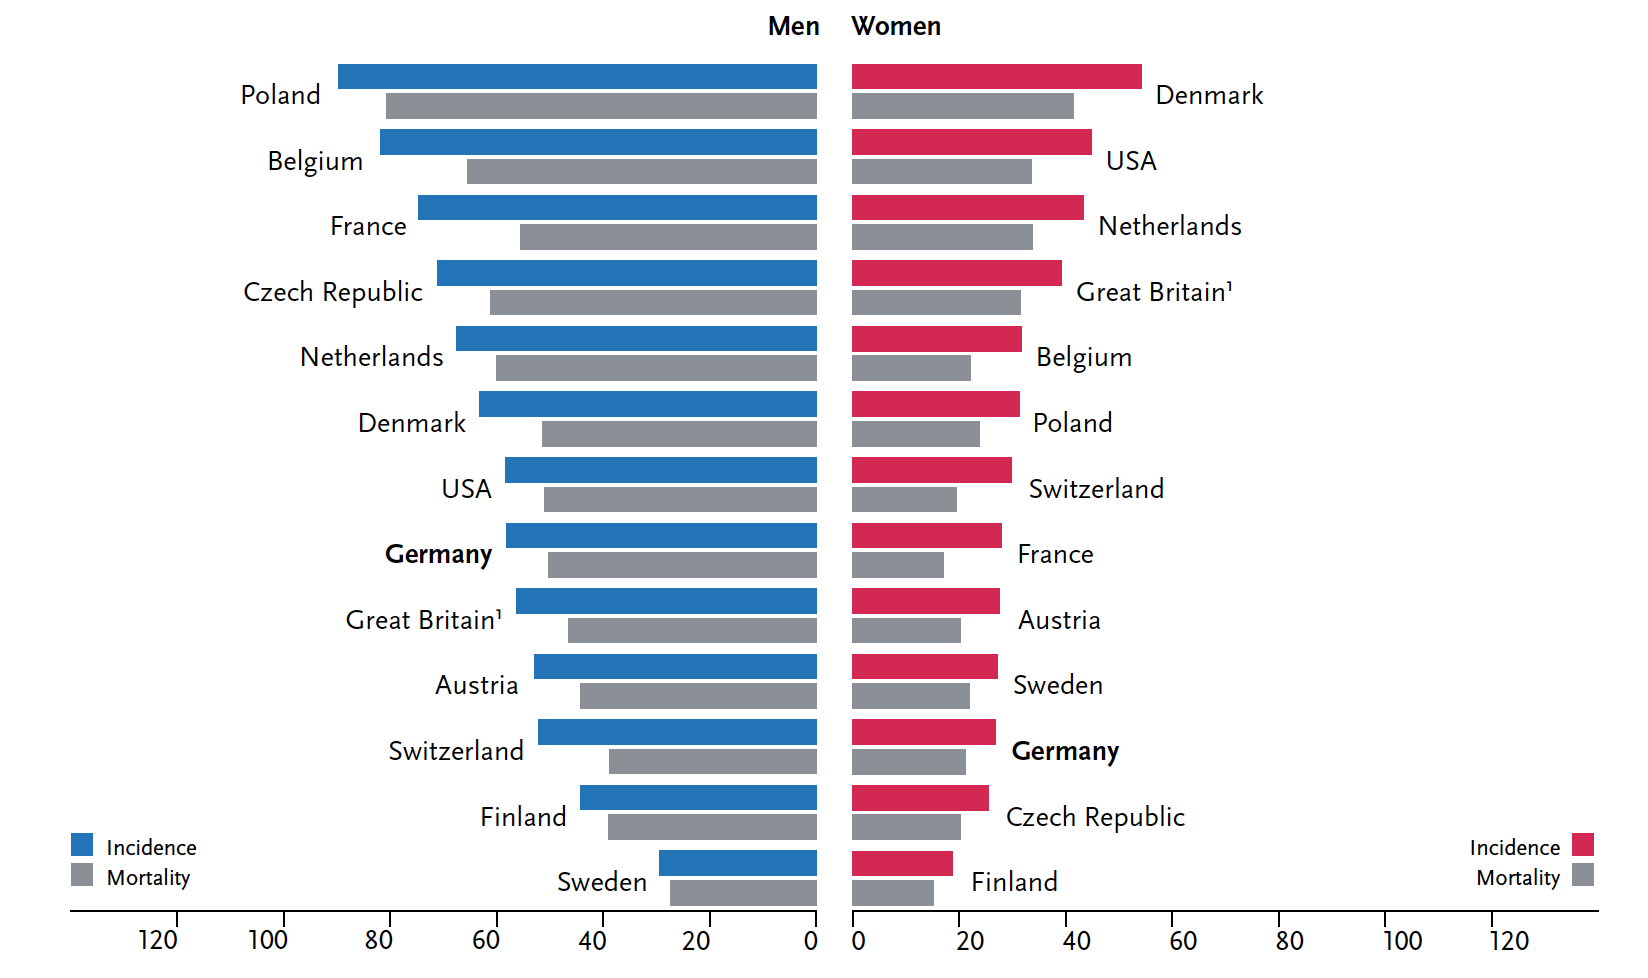
\includegraphics[width=\textwidth]{cancerInternational.png}
\caption{International comparison of age-standardized incidence and mortality rates for lung cancer in the year 2012}
\label{fig:cancInt}
\end{figure}

The main risk factor has been shown to be the exposure to tobacco smoke, whether it's active consumption via cigarettes, or passive exposure especially in closed rooms. CT scanners are used to detect irregular tissue in a patients lung region. These irregularities are grouped under the term \textit{pulmonary nodule}. A pulmonary nodule is a small, round (parenchymal) or worm (juxtapleural) shaped lesion in the lungs. Each lesion has a chance to be malignant and may grow and spread over time, becoming a risk for the patient's life in the form of lung cancer. Nodules come not only in different shapes but differ along other features as well. Ground-glass opacity (GGO) nodules are a challenging kind of nodules since they are not thoroughly solid and so harder to detect on a CT scan. The location of the nodules is crucial for the detection rate since nodules close to bigger vessels or the chest wall do not differ much in intensity to the surrounding tissue and can be easily overlooked by the radiologist.


\section{Current Medical Approach}
In the clinical setting, the supervising medical staff has additional information available apart from the CT scans. Patients are either in a high-risk group (over a certain age and heavy smokers) or present certain syndromes like fatigue, weight loss, cough, dyspnea, hemoptysis and chest pain. Different methods are used to find the underlying cause of these symptoms:

\begin{description}
\item[Sputum cytology] Sputum is mucus that is produced in the lower airways which can be analyzed for bacteria and irregular cells.
\item[Biopsy] In a biopsy tissue samples are directly taken from the lung of the patient. This may be done in several ways, either bronchoscopic (obtaining the sample with an instrument through the airways) or directly by a needle or incision through the chest wall.
\item[Imaging tests] different imaging techniques are available for analyzing the lung: a regular X-Ray scan, but also MRI. The data used in this thesis stems from LDCT scans which stand for \emph{low-dose computed tomography}. The radiation used in this method lies around 2.35 mSv which corresponds to roughly 80$\%$ less radiation then regular CT scans \cite{ono2013low}.
\end{description}

Lung cancer is tricky to detect since the symptoms show up very late in the process of the illness and it is often too late for the patient when those are recognized. Sputum cytology and biopsy are only used when there is already circumstantial evidence (like other symptoms) for lung cancer which may often be too late in the development of the illness for a successful treatment. This makes imaging techniques the only source for early detection. Radiologists are required to analyze roughly 100-600 pictures per patient depending on the slice thickness of the used technique and the body height of the patient. Medical image viewers like OsiriX \ref{fig:osirix} are assisting in this process and have also been used in this thesis to analyze the image data.

\begin{figure}[ht]
\includegraphics[width=\textwidth]{Osirix_program.png}
\caption{Screenshot of the analyzing software OsiriX. It is the most widely used software in the domain of medical image viewers and offers a free trial version that was used for this thesis.}
\label{fig:osirix}
\end{figure}

Yet it is still a highly complicated task and despite all efforts in this field the process is of course not fail-safe and it can happen that nodules are not detected in an early stage of their development but later when a successful treatment is not as likely anymore. A study by Kakinuma et. al.\cite{kakinuma2012comparison} shows how different features like the slice thickness and the nodule properties affect the detection rate, dropping it to 65.5$\%$ for pure ground-glass opacities in a scan with 2mm slice thickness. Another issue arises with the false positive rate. A study by Pinsky et. al.\cite{pinsky2013national} reports a mean false positive rate of 28.7$\%$ across 112 radiologists at 32 screening centers in and outside of the US. This puts additional stress on the patient and requires further tests to conclude that there is no cancer present.


\section{Opportunities for Assistance}

Early detection of lung cancer is important in two ways. First, it increases the chance of a successful treatment and secondly, it avoids unnecessary scans in the scenario of undetected cancerous material or wrongly classified abnormalities in the lung. As the number of preventive screening procedures rises and the used scanners become more granular software-based assistance becomes a helpful companion to every radiologist \cite{li2005computer}.

The scientific literature provides many algorithmic approaches to finding nodules in CT Scans \cite{armato1999computerized}\cite{armato2001automated}\cite{okada2005robust}\cite{tao2009multi}\cite{ye2009shape} using handcrafted features and in-depth knowledge of the structure of the data and the nodules that should be detected. Some make already use of Deep Convolutional Neural Networks to solve this or related tasks (like classifying the malignancy of a nodule) \cite{cheng2016computer}\cite{huang2017lung}\cite{shen2015multi}.

Despite many efforts being devoted to the computer-aided nodule detection problem, lung CAD systems remain an ongoing research topic. One of the major difficulties is the detection of GGO nodules with low-dose thin-slice CT screening. Another two difficulties are the detection of nodules that are adjacent to vessels or the chest wall when they have very similar density and the detection of nodules that are nonspherical in shape. In such cases, classical approaches like intensity thresholding or model-based methods might fail to identify the nodules correctly.

\section{The Problem of Neural Networks}
Neural Networks are strong tools that \emph{solve} many tasks with astonishing performance (see for example \cite{silver2017alphagozero}). Yet it seems like the solution they come up with is not intelligible to humans in the same way as (for example) a feature detector that was directly designed to respond to geometric properties of the nodule. But in a scenario where medical decisions are based on the output of an algorithm, it is crucial that the algorithm is reliable and the way it comes up with a decision is accepted by the people responsible. As long as this is not the case the people working with the software will not completely accept its value and it can not be ruled out that the network produces erroneous results in cases that did not occur during the training phase.

In this thesis, a Deep Neural Network will be developed that uses 3D CT scan information to classify a given CT image patch as either containing a nodule or not. Then mechanisms will be applied to visualize the learned features and discussed whether they can be conceptualized in terms of already approved procedures. The problem in this sense is two-fold. First - can a 3D Convolutional Neural Network solve the task of nodule detection and second, how can it's solution to the problem be understood? 


\section{Structure of this thesis}
This thesis is structured in the following way: in chapter \ref{chap:02data} the used dataset is described as well as it's preprocessing for the learning algorithm. The methods chapter (\ref{chap:03methods}) contains information about the used software packages that were necessary to implement the algorithms as well as information about Convolutional Neural Networks and the learned model that is analyzed in chapter \ref{chap:04results}. That chapter focuses on extracting the features from the convolutional kernels and compares them to traditional approaches. In chapter \ref{chap:05discussion} the results are revised and items for further investigation and optimization are presented together with a more general outlook on the topic of analyzing Neural Networks to gain insights into problems and not just as solutions to them. 

\end{document}
